\section{Definitions and Notations}
\label{sec:preliminaries}

\subsection{Useful definitions}

Two $k$-cliques are \emph{neighbours} if they share $k-1$ nodes.

For a given graph $G$, and a $k$-clique $c_k$, let $\mathcal{N}(c_k)$ be the the of $k$-cliques neighbours of $c_k$, that is to say the set of $k$-cliques of $G$ which share $k-1$ nodes with $c_k$.

A $path$ between two $k$-cliques $c_0$ and $c_n$ is a set of $k$-cliques $c_1, ..., c_{n-1}$ such that for $1 \leq i \leq n$, $c_i$ and $c_{i-1}$ are neighbours, that is they share $k-1$ nodes.

A $k$-clique community is a maximal set of $k$-cliques such that there is a path between each pair of $k$-clique.

In an recursive point of view, we can define a $k$-clique community $\mathcal{C}$ as : $\mathcal{C} = \underset{\substack{k-clique \\ c_k \in \mathcal{C}}}{\bigcup} \mathcal{N}(c_k)$. It gives a naïve way to build a community : starting from a $k$-clique and extending to its neighbours until the community stops growing.

\subsection{The clique percolation method (CPM) problem}
\label{subsec:defcpm}

The problem in which we worked during this internship is the \emph{k-Clique Percolation Method (CPM)} problem. This problem outputs a way to group the nodes which are ``close'' to each other, in a way we define just below.

The goal of this work is to partition the $k$-cliques of a given graph into communities. The input is a graph $G$ (a list of edges), and the output is a list of set of nodes, each one corresponding to a $k$-clique community of the graph.

The notion of $k$-clique communities allows to group nodes into overlapping sets which be analysed to show there different characteristics. Figure \ref{fig:palla} and Figure \ref{fig:kumpula} are from Palla [REF] and Kumpula [REF] papers, and they show illustrations of graph $k$-clique communities and its interesting overlapping.

\begin{figure}[h]
  \centering
  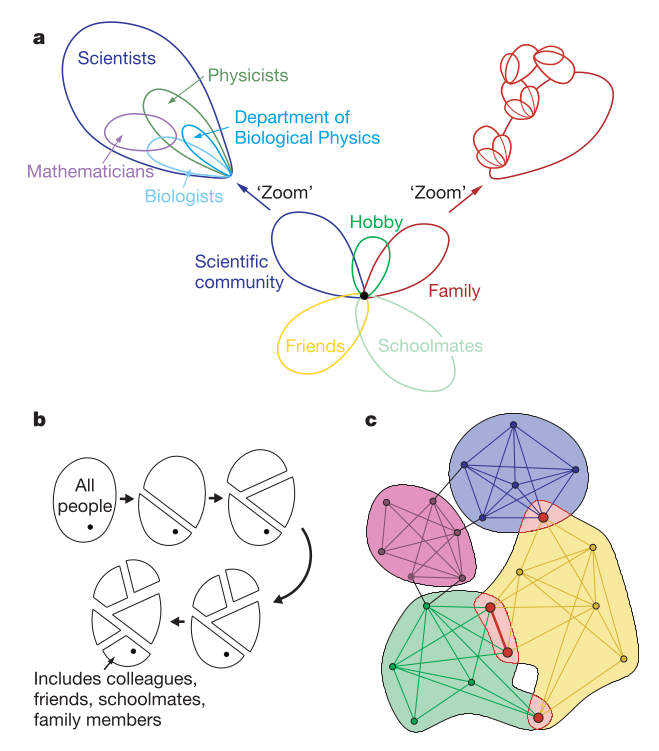
\includegraphics[scale=0.45]{Contents/commusPalla}
  \caption{Illustration of the concept of overlapping communities, from Palla's paper [REF].}
  \label{fig:palla}
\end{figure}

\begin{figure}[h]
  \centering
  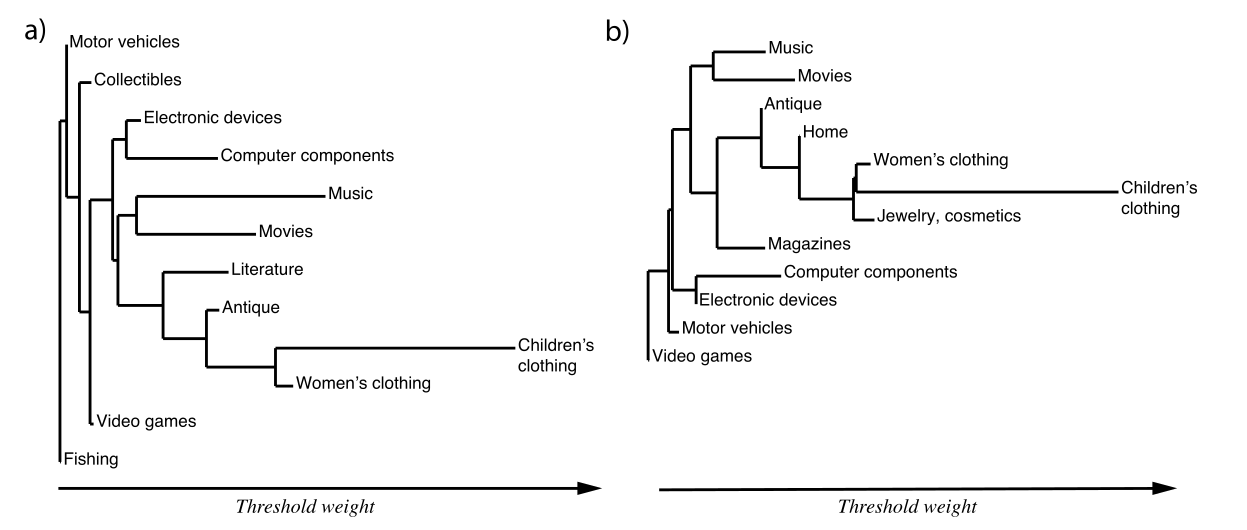
\includegraphics[scale=0.35]{Contents/commusKumpula}
  \caption{Dendogram visualization of $k$-clique communities to show the overlapping interest. Dendograms are from Kumpula paper [REF].}
  \label{fig:kumpula}
\end{figure}

We generalize the term of \emph{$k$-clique community}. In this report, we talk about community without necesarily having the maximality property. Each set of $k$-clique in which there is a path between any $k$-clique to any other, with the definition given in section~\ref{subsec:defcpm}, is called a community. Because in our algorithms communities are build little by little, it allows us to name communities in the algorithm, before they are maximal at the end of the algorithm.

% ...

% $n_k$ denotes the number of $k$-cliques.

% $T_k$ denotes the time to list all $k$-cliques.
